\mychapter{Nombres Racionals}
{Nombres Racionals}
{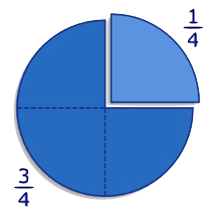
\includegraphics[width=4cm]{img1/image1.png}}
{chap:racionals}
 
\vspace{1cm}
\begin{iniaval}
	\textbf{Completa:}
	
	\begin{itemize}
		\item En una fracció $\frac{a}{b}$, $a$ es diu ................................... i $b$ s'anomena \dotfill
		
		\item  Quan una fracció no es pot simplificar més es diu \dotfill
		
		\item  Quant val les dues terceres parts de 24?  \dotfill
		
		\item  Una botella de vi de 3/8 de litre; com s'expressa com a número decimal? \dotfill
	\end{itemize}
	
	\vspace{0.5cm}
	\textbf{Calcula i simplifica:}
	
	\begin{tasks}(2)
		\task $\frac{3}{4}+\frac{7}{2}-3=$    \task $\frac{3}{7}\cdot\frac{28}{6}=$
		
		\task $\frac{3}{4}:\frac{7}{2}=$      \task $\frac{3}{7} \text{ de } 42=$
	\end{tasks}	

	\vsoo
	\addanswersline{Avaluació inicial}{0}{$a$: numerador,\par $b$: denominador,\par irreductible,\par $\frac{2}{3} \text{ de } 24=16$,\par $\frac{3}{8}=0.375$ litres,\par
	\begin{tasks}(2)
			 \task $\frac{5}{4}$ \task $2$ \task $\frac{3}{14}$ \task $18$
	\end{tasks}	
	}
\end{iniaval}



\newpage
\section{Operacions amb nombres enters}

\begin{theorybox}[Prioritat de les operacions]
	\begin{tabular}{ll}
		& $3 - (-2)^{2} \cdot ( 4 - 9)$ \\
		\textbf{1r} Efectuam els parèntesi          &     $ 3 - (-2)^{2} \cdot (-5)$ \\
		
		\textbf{2n} Calculam potències i arrels        &    $ 3 - 4 \cdot (-5)$     \\
		
		\textbf{3r} Efectuam les multiplicacions i les divisions &  $ 3 + 20$ \\
		
		\textbf{4t }Finalment, feim les sumes i les restes.       &                      $23$
	\end{tabular}
\end{theorybox}

\begin{mylist}
	\exer  \spen  Calcula:

\begin{tasks}(2)
	\task  $-2 \cdot (-20 + 15)  =$    
	
	\task  $-20 : \left(10 - 2\cdot (-20 + 15) \right) =$      
	
	\task*(2) $\left[-80 -20 : \left(10 - 2\cdot (-20 + 15) \right) \right] \cdot (3 - 2 \cdot 3^{2})$=
	
\end{tasks}
\vso
 	\answers{[$10$, $-1$, $1215$]}



	\exer  \spen  Calcula pas a pas:   $(-5 + 4 \cdot (-2) +7) : (7 - (3 - 4)\cdot (-1))$
\vsoo
	\answers{$-1$}







	\exer  \spen  Calcula:

\begin{tasks}(2)
	\task $-10 + 20 : (-5) =$ 
 
	\task $-100 : \left[ (-20) : (-5) \right]=$ 
 
\end{tasks} 
\answers{[$-14$, $-25$]}



	
\exer[1]  Calcula:

\begin{tasks}(2)
\task $3-(4\cdot 3-2\cdot 5)^{2} -(3-5)^{3} $   \task $5-3^{2} -2\cdot (-5)-(7-9)^{2} $
\task $7-2\cdot (3-5)^{2} +2\cdot (-3)+8-(-2)^{2} $  \task $2-(2\cdot 3-3\cdot 4)^{2} -(2-4)^{3} $
\end{tasks} 
\answers[cols=2]{[$7$, $2$, $-3$, $-26$]}

\end{mylist}

\section{Operacions amb nombres racionals}

\begin{theorybox} 
\begin{multicols}{2}
	\centering
\videonw[ytid=ZzRAv1IAUig]{117}{Nombres racionals, operacions simples.}
\videonw[ytid=GX7auykiAA4]{118}{Nombres racionals, operacions combinades.}  
\end{multicols}
\end{theorybox}

\vspace{2cm}

\begin{mylist}
	
\exer[1] \spen Calcula i simplifica.
 
\begin{tasks}(2)
\task $\frac{3}{2} -\frac{3}{10} -\frac{3}{5} =$                \task  $\frac{7}{12} +\frac{4}{9} -\frac{1}{2} +\frac{3}{4} -\frac{7}{6} =$  

\vsoo

\task $\frac{1}{2} -\frac{3}{4} -\frac{2}{3} +1=$                \task $\frac{1}{11} -\frac{13}{22} -\frac{1}{4} +1=$

%\vsoo

%\task  1 -- $\frac{2}{3} +\frac{2}{5} -\frac{7}{5} =$               \task$\frac{4}{7} +\frac{1}{2} -\frac{8}{21} -\frac{5}{14} =$
\end{tasks}
\vsooo
\answers[cols=2]{[$\frac{3}{5}$, $\frac{1}{9}$, $\frac{1}{12}$, $\frac{1}{4}$]}

 
\exer[1] \spen  Calcula i simplifica.
 
 \begin{example}
 	 a) $\ \ \frac{7}{6} - \left(\frac{1}{2}-\frac{1}{3}\right)=\frac{7}{6}-\left(\frac{3}{6}-\frac{2}{6}\right)=\frac{7}{6}-\frac{1}{6}=\frac{6}{6}=1$
 	 \vspace{0.25cm}
 \end{example}

\begin{tasks}(2)
\task$\frac{7}{6} -\left(\frac{1}{2} -\frac{1}{3} \right)$=                   \task $2-\left(\frac{1}{2} -\frac{1}{3} \right)$=               
\vsoo

\task $\frac{6}{7} -\left(\frac{3}{7} -\frac{11}{14} \right)$=                    \task $\left(\frac{5}{6} +\frac{2}{5} \right)$$-\left(\frac{3}{5} +\frac{1}{6} \right)$=             
\vsoo

\task $\left(\frac{3}{4} +\frac{2}{5} +1\right)-\left(2-\frac{7}{5} \right)$=                 \task $\left(5-\frac{7}{2} \right)-\left(3+\frac{1}{4} \right)+\left(2-\frac{3}{8} \right)$ =
\vsoo

\task $\left(1+\frac{1}{2} +\frac{1}{4} \right)-$$\left(1+\frac{1}{3} +\frac{1}{6} \right)$=          \task $\left(\frac{11}{12} -\frac{3}{4} +\frac{1}{8} \right)-\left(\frac{1}{2} -\frac{2}{3} -\frac{5}{4} \right)$=
\end{tasks}
\vsooo
\answers[cols=2]{[$1$, $\frac{11}{6}$, $\frac{17}{14}$, $\frac{7}{15}$, $\frac{31}{20}$, $-\frac{1}{8}$, $\frac{1}{4}$, $\frac{41}{24}$]}


 
\exer[1]  Opera i simplifica.
 
\begin{tasks}(2)
\task $2\cdot \left(\frac{1}{2} -\frac{1}{6} \right)$=         \task $2:\left(\frac{1}{2} -\frac{1}{4} \right)$  =

\task $\left(\frac{2}{5} -\frac{1}{3} \right)\cdot 5$   =       \task $\frac{3}{7} :\left(1-\frac{1}{7} \right)$ =

\task  $\left(\frac{1}{2} +\frac{1}{4} \right)\cdot \left(1-\frac{1}{3} \right)$ =      \task$\left(1-\frac{1}{5} \right):\left(\frac{1}{2} +\frac{3}{10} \right)=$

\task $\left(5-\frac{1}{2} -\frac{7}{3} \right):\left(\frac{6}{5} -\frac{1}{3} \right)=$     \task $\left(1+\frac{1}{2} +\frac{1}{8} \right)\cdot \left(2-\frac{10}{13} \right)=$

\task $3\cdot \left(\frac{1}{2} +\frac{1}{3} \right)-2\cdot \left(2-\frac{1}{3} \right)=$                          \task $\frac{1}{2} \cdot \left(1+\frac{2}{5} \right)+2\cdot \left(1-\frac{3}{5} \right)=$

\task $\frac{2}{3} \cdot \left(\frac{1}{2} +\frac{2}{3} \right)-2\cdot \left(\frac{2}{3} -\frac{4}{9} \right)=$   \task $\frac{3}{4} \cdot \left[\frac{6}{5} -\frac{2}{7} \cdot \left(1+\frac{2}{5} \right)\right]$=
\end{tasks}
\answers{[$\frac{2}{3}$, $8$, $\frac{1}{3}$, $\frac{1}{2}$, $\frac{1}{2}$, $1$, $\frac{5}{2}$, $2$, $-\frac{5}{6}$, $\frac{3}{2}$, $\frac{1}{3}$, $\frac{3}{5}$]}
 
 \begin{comment}
	\exer  La mitjana harmònica es defineix com a $H(a,b)=\frac{1}{\frac{\frac{1}{a}+\frac{1}{b}}{2}}$, l'invers de la mitjana aritmètica dels inversos.
 

a) Demostra que H(a, b) = $\frac{2ab}{a+b} $  \quad\quad  b) Troba $H\left(\frac{3}{2} ,\frac{11}{3} \right)$ 
\end{comment}
 
	\exer \spen Troba la fracció inversa de $\mathrm{3+}\frac{\mathrm{4}}{\mathrm{5}}\mathrm{:}\frac{\mathrm{6}}{\mathrm{10}}=$
	\answers{$\frac{3}{13}$}
	
	\exer  \spen Opera i simplifica: $\frac{4}{5} \cdot \frac{6}{14} \cdot \frac{10}{12} \cdot \frac{7}{2}=$
	\answers{$1$}
	
	\exer  Resol pas a pas  $\frac{\frac{\mathrm{3}}{\mathrm{5}}\mathrm{-}\frac{\mathrm{2}}{\mathrm{5}}\mathrm{:}\frac{\mathrm{4}}{\mathrm{6}}}{\frac{\mathrm{3}}{\mathrm{5}}\mathrm{:}\left( \frac{\mathrm{1}}{\mathrm{6}}\mathrm{-}\mathrm{2}\right)}=$ 
	\answers{$0$}
	
	\exer \spen Simplifica:  
	\begin{tasks}(2)
	\task $\; \frac{2\cdot 7\cdot 15}{21\cdot 10} = \quad \quad \quad$
	
	%%\task $\; \frac{10+6}{10-2} \quad \quad \quad$ 
	
	\task $\; \frac{2\cdot 3+4}{2\cdot 5+10}= $
	\end{tasks}
	\answers[cols=2]{[$1$, $\frac{1}{2}$]}

	\exer[1]  Calcula: 
 \begin{tasks}(3)
 	\task $\frac{2}{3} \cdot \left(\frac{3}{2} :\frac{1}{3} \right)^{2} +\left(2-\frac{1}{2} \right)^{2} $ 
 	\task $\frac{3}{4} \cdot \left(\frac{3}{2} :\frac{3}{4} \right)^{3} +\left(2-\frac{3}{2} \right)^{2} $ 
 	\task $\frac{8}{3} \cdot \left(\frac{3}{4} :\frac{1}{2} \right)^{2} +\left(\frac{1}{2} -1\right)^{3} $ 
 \end{tasks}
 \answers[cols=2]{[$\frac{67}{4}$, $\frac{25}{4}$, $\frac{47}{8}$]}


\end{mylist}

\newpage
\section{Representació de fraccions sobre la recta numèrica}
 
\begin{theorybox}
\video[rows=4,ytid=FXWcB8irMk8]{153}{Representació de fraccions \vspace{-0.5cm}}

\textbf{Classificam les fraccions en tres tipus:}

- Fraccions \textbf{pròpies} (menors que la unitat): $\frac{1}{2},\frac{2}{3},\frac{5}{9},$ ···

- Fraccions \textbf{iguals a la unitat}: $\frac{2}{2},\frac{3}{3},\frac{4}{4},$ ···

- Fraccions \textbf{impròpies} (majors que la unitat): $\frac{7}{2}, \frac{11}{3}, \frac{-49}{5}, \cdots$·

Les fraccions impròpies es poden expressar com un\textbf{ número mixt}:  
$\frac{7}{3}=\ 2\ +\frac{1}{3}$

\end{theorybox}


\begin{mylist}
	\exer \spen  Passa a forma mixta les següents fraccions: $\frac{50}{7} ;\frac{25}{11} ;\frac{101}{6} $
 \vsooo
	\answers[cols=2]{[$7+\frac{1}{7}$, $2+\frac{3}{11}$, $16+\dfrac{5}{6}$]}
 
	\exer \spen Passa a forma mixta les fraccions $\frac{-30}{7} ;\frac{-50}{13} ;\frac{-100}{21} $ 
 \vsooo
	\answers[cols=2]{[$-4-\dfrac{2}{7}$, $-3-\dfrac{11}{13}$, $-4-\dfrac{16}{21}$]}
 
	\exer \spen Representa en la recta numèrica les fraccions: $\frac{1}{5} ;\frac{3}{7} ;\frac{-5}{8} ;\frac{-3}{4} $ 
	\begin{center}
	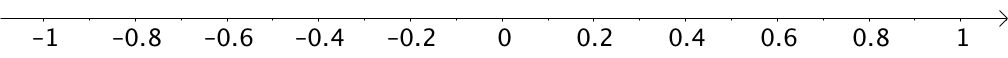
\includegraphics[width=0.9\textwidth]{img1/rectanum11}
	\end{center}
	\answers{Gràfica:\par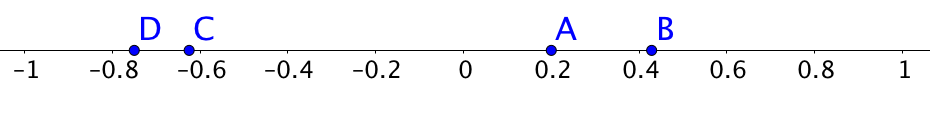
\includegraphics[width=0.45\textwidth]{img-sol/t1-recta1}}
 \vsooo
 
	\exer \spen Passa a forma mixta i representa les fraccions: $\frac{23}{8} ;\frac{-23}{8} ;\frac{180}{50} ;\frac{-26}{6} $ 
	\begin{center}
		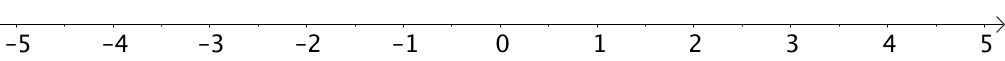
\includegraphics[width=0.9\textwidth]{img1/rectanum}
	\end{center}
	\answers{Gràfica:\par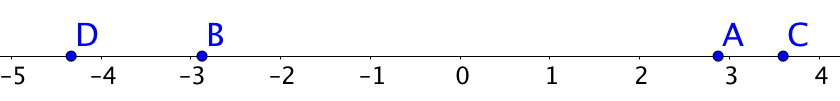
\includegraphics[width=0.45\textwidth]{img-sol/t1-recta2}}
 \vsooo
\newpage
 
	\exer \spen  Troba les fraccions que es corresponen amb els punts \textit{A, B, C, D} i \textit{E, }expressant\textit{ }en forma mixta i com a fracció impròpia les representades pels punts \textit{A, B} i \textit{E}.
 
\includegraphics*[width=0.93\textwidth]{img1/image4.png}

A=\quad\quad\quad\quad\quad\quad B=\quad\quad\quad\quad\quad\quad  C=\quad\quad\quad\quad\quad\quad  D=\quad\quad\quad\quad\quad\quad E=\quad\quad\quad\quad\quad\quad
 \vsooo
 \answers{$A=-2-\dfrac{2}{9}=-\dfrac{20}{9}$;\par $B=-1-\dfrac{6}{8}=-\dfrac{14}{6}$;\par $C=-\dfrac{3}{4}$;\par $D=\dfrac{3}{5}$;\par $E=2+\dfrac{4}{7}=\dfrac{18}{7}$}

\end{mylist}

\section{Fraccions i decimals}
 
\begin{theorybox}
\video[ytid=12GEHAqGpzA]{119}{Nombres racionals: Relació entre fracció i decimal.}

Els nombres decimals es classifiquen en: 

- \textbf{Exactes}:  com $1,25=\ \frac{125}{100}$

- \textbf{Periòdics}:   Són Fraccions
	
	\quad\quad\quad \textbf{Pur}$\boldsymbol{:}\ 3,626262\textrm{·}\textrm{·}\textrm{·}=3,\widehat{62}$ $=\ \frac{362-3}{99}=\frac{359}{99}$               

	\quad\quad\quad \textbf{Mixt: }$7,19999\textrm{·}\textrm{·}\textrm{·}\textrm{·}=7,1\hat{9}=\frac{719-71}{90}=\frac{648}{90}$

\textbf{- No periòdics}: com el número $\pi$, $\sqrt{2}, \cdots$. No són fraccions.
\end{theorybox}




\begin{mylist}
	\exer  Sense fer la divisió indica si les següents fraccions tenen expressió decimal exacta o periòdica:
 
\begin{tasks}(4)
	\task  $\frac{21}{750} $ 
	\task $\frac{75}{21} $
	\task $\frac{11}{99} $
	\task $\frac{35}{56} $
\end{tasks} 
	\answers[cols=2]{[Exacte, Periòdic, Periòdic, Exacte]}

\textit{Ajuda}: \textit{La divisió és exacta només quan la descomposició del denominador conté únicament 2 o 5.}

 
	\exer Passa a fracció i simplifica:
	\begin{tasks}(3)
		\task 1,4142  
		\task 0,125 
		\task 6,66
	\end{tasks}
 	\answers{[$\dfrac{7071}{5000}$, $\dfrac{1}{8}$, $\dfrac{333}{50}$]}
	
	\exer Passa a fracció i simplifica:
 \begin{tasks}(3)
 	\task 1,41424142{\dots}  
 	\task 0,125125{\dots} 
 	\task 6,666{\dots}
 \end{tasks}
	\answers{[$\dfrac{14141}{9999}$, $\dfrac{125}{999}$, $\dfrac{20}{3}$]}
 
 
	\exer  Passa a fracció i simplifica:
 \begin{tasks}(3)
 	\task 1,04444{\dots} 
 	\task  0,7125125{\dots}
 	\task  6,7666{\dots}
 \end{tasks}
	\answers{[$\dfrac{47}{45}$, $\dfrac{3559}{4995}$, $\dfrac{203}{50}$]}

\vspace{2cm}
 
	\exer  \spen  Completa la taula següent
 
\begin{tabular}{|p{0.28\textwidth}|p{0.28\textwidth}|p{0.28\textwidth}|} \hline 
	\rowcolor{lightgray} Decimal & Fracció & Percentatge \% \\ \hline 
	0,75 &  &  \\ \hline 
	& 6/4 &  \\ \hline 
	&  & 68\% \\ \hline 
\end{tabular}
\answers{
	{\renewcommand{\arraystretch}{1.8}
	\begin{tabular}{|c|c|c|} \hline 
		\rowcolor{lightgray} Decimal & Fracció &  \% \\ \hline 
		0,75 &  $\frac{3}{4}$ & 75 \%  \\ \hline 
		1,5 & $\frac{6}{4}$ & 150 \% \\ \hline 
		0,58 & $\frac{17}{25}$ & 68\% \\ \hline 
	\end{tabular}}
}

 
	\exer  Calcula el número decimal que correspon al percentatge 130\% i el percentatge que correspon a la fracció 7/25.
 \answers{$130$ \%=$0.13$ i $\frac{7}{25}=28$ \%}


 
\exer[1]  Calcula, passant prèviament a fracció cada nombre decimal: 
 \begin{tasks}(3)
 	\task 0,333{\dots} + 0,666{\dots} 
 	\task 0,888{\dots} $\cdot$ 2,5
 	\task 0,65 : 0,656565{\dots}
 \end{tasks}
\answers[cols=3]{[$1$, $\dfrac{20}{9}$, $\dfrac{99}{100}$]}

\end{mylist}

\begin{example}
 
$\mathrm{1,66666\textrm{·}\textrm{·}\textrm{·}\ -\ 1,0222\textrm{·}\textrm{·}\textrm{·}\ =1,}\widehat{\mathrm{6}}\mathrm{-}\mathrm{1,0}\widehat{\mathrm{2}}\mathrm{=}\frac{\mathrm{16-1}}{\mathrm{9}}\mathrm{-}\frac{\mathrm{112-10}}{\mathrm{90}}\mathrm{=}\frac{\mathrm{15}}{\mathrm{9}}\mathrm{-}\frac{\mathrm{102}}{\mathrm{90}}\mathrm{=}\frac{\mathrm{48}}{\mathrm{90}}\mathrm{=}\frac{\mathrm{8}}{\mathrm{15}}$
\vspace{0.25cm}
\end{example}


\begin{mylist} 
 
	\exer  Demostra que 4,999{\dots} = 5. Generalitza: Quant val n,999{\dots}?
 
 	\answers{$4,999{\cdots}=4,\hat{9}=\frac{49-4}{9}=\frac{45}{9}=5$.\par En general:
 	$n,999{\cdots}=n,\hat{9}=\frac{10n+9-n}{9}=\frac{9n+9}{9}=n+1$
 }


 
	\exer  Representa de forma exacta en la recta numèrica: $\frac{760}{240};\ \ 3,125;\ -\frac{46}{14}$; -2,1666{\dots}
	
	\answers{Gràfica:\par 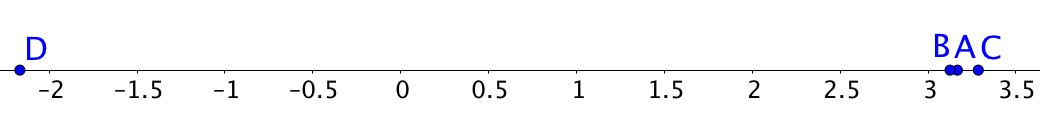
\includegraphics[width=0.5\textwidth]{img-sol/t1-recta3}}
\end{mylist}

\section{Ordenar fraccions}
 

\begin{theorybox}
\video[ytid=I6Arx0Z6o2M]{152}{Nombres racionals.}  

\textbf{Per ordenar fraccions ho podem fer de dues formes diferents:}

- Reduir les fraccions a denominador comú (mín. c. m.)

- Convertir les fraccions a nombre decimal i ordenar els números decimals
\vspace{0.25cm}
\end{theorybox}

\begin{mylist}
	 

 
	\exer  Ordena de menor a major: $\frac{7}{12},\frac{4}{6},\frac{5}{9},\frac{3}{4},\frac{13}{18}$

\end{mylist}	

	\begin{example}[*]
		\textbf{Primer mètode}: Reduir a denominador comú.
				$min.c.m(12, 6, 9, 4, 18) = 36$
		
		$\frac{7}{12},\frac{4}{6},\frac{5}{9},\frac{3}{4},\frac{13}{18}$  \quad $\rightarrow$ \quad $\frac{21}{36},\frac{24}{36},\frac{20}{36},\frac{27}{36},\frac{26}{36}$
		
		Ordenam de menor a major les fraccions originals $\frac{5}{9} < \frac{7}{12} < \frac{4}{6} < \frac{13}{18} < \frac{3}{4}$
		
		\textbf{Segon mètode}: Valor decimal
		
		$\frac{7}{12},\frac{4}{6},\frac{5}{9},\frac{3}{4},\frac{13}{18}$  \quad $\rightarrow$ \quad $0.8\hat{3}, 0.\hat{6}, 0.\hat{5}, 0.75, 0.7\hat{2}$
		
		i ordenam els nombres decimals de menor a major i trobam el mateix resultat que abans.
		
	\end{example}
 


\begin{mylist}


	\exer  Ordena de menor a major: $\frac{8}{9} ;\frac{-8}{9} ;\frac{4}{5} ;\frac{38}{45} ;\frac{77}{90} ;\frac{-9}{8} $
	\answers{$\frac{-9}{8}< \frac{-8}{9}<\frac{4}{5} <\frac{38}{45} <\frac{77}{90}  < \frac{8}{9}$}


 
	\exer  Ordena de menor a major: $\frac{11}{24},\ -\frac{7}{4},\frac{3}{8},\ -\frac{1}{6},\frac{5}{12},\ -\frac{5}{3}$
 \answers{$-\frac{7}{4}<-\frac{5}{3}<-\frac{1}{6}<\frac{3}{8}<\frac{5}{12}<\frac{11}{24}$}
 



 
	\exer  Suposa que tens dues fracció $a$ i $b$ i vols trobar el nombre que es troba just enmig. Explica com ho faràs. Inventat un exemple i representa les tres fraccions sobre la recta numèrica.
	
	\redacta
	\answers{El que començam fent és sumar les dues fraccions $a$ i $b$. Després el resultat en dividim entre dos. D'aquesta forma tenim el nombre que està enmig. Per exemple: si $a=\frac{2}{3}$ i $b=\frac{5}{4}$,
	\[\frac{2}{3} +\frac{5}{4} =\frac{8}{12} + \frac{}{12} = \frac{23}{12} \]	
	Finalment dividim entre dos: La fracció és $ \frac{23}{24} \approx 0,958\hat{3}$
	\par
	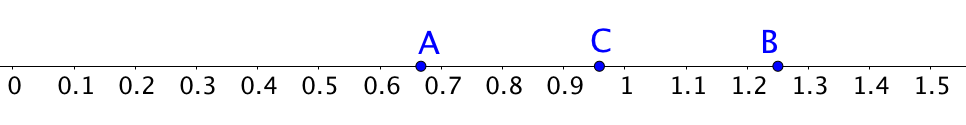
\includegraphics[width=0.5\textwidth]{img-sol/t1-recta4}
}
\end{mylist}
 
\section{Problemes de fraccions}
\begin{theorybox} 
\begin{minipage}{0.5\textwidth}
	\centering
	\videonw[ytid=o9DhLJxyPz0]{120}{Nombres racionals: Problemes tipus Part-Fracció-Total}
\end{minipage}
\begin{minipage}{0.5\textwidth}
	\centering
	\videonw[ytid=O9HQD38HBL8]{154}{Nombres racionals: Problemes típics amb fraccions}
\end{minipage}


\textbf{- Recorda l'essencial:}
\[\text{Fracció} = \frac{Part}{Total} \quad\quad\quad Part=\text{Fracció} \cdot Total   \quad\quad\quad  Total = \frac{Part}{\text{Fracció}}\]
\textbf{- Totes les fraccions de les parts sumen 1}

\end{theorybox}

\begin{mylist}
	\exer \spen  Calcula les dues terceres part de la sisena part del 80\% de 900.
 \vso
 \answers{80}

 
	\exer  \spen  Troba el nombre tal que els seus quatre terços valen 520.
 \vsoo
\answers{390}



 
	\exer  \spen  Quants pots de tres vuitens de litre puc omplir amb 12 litres?
 \vso
\answers{32 pots}
 
	\exer  Inventat un problema on aparegui la fracció $\frac{2}{5}$ i el nombre $200$. Resol aquest problema i comparteix-lo amb el teus companys. 
	 
	 \answers{Per exemple: En el nostre institut les $\frac{2}{5}$ parts dels alumnes de 3r d'ESO són d'Alaró. Si en total hi ha $200$ alumnes a 3r d'ESO, quants són d'Alaró?\par
	 \par Solució: $\frac{2}{5}$  de $200$ = 80 alumnes són d'Alaró.}  
\redacta

\pagebreak
\mbox{}
\vspace{-1cm} 
 
 \exer \begin{minipage}[t]{0.56\textwidth}  Si 100 polzades són 254 cm:
 
\begin{tasks}
	\task Troba el llarg en centímetres d'una televisió si l'altura són 19,2 polzades i llarg/alt = 4/3
	\task Igual però ara llarg/alt = 16/9
\end{tasks}
\answers{[65.024 cm, 86.6986 cm]} 

\end{minipage}
\begin{minipage}{0.44\textwidth}
	\centering
	\vspace{0.5cm}
	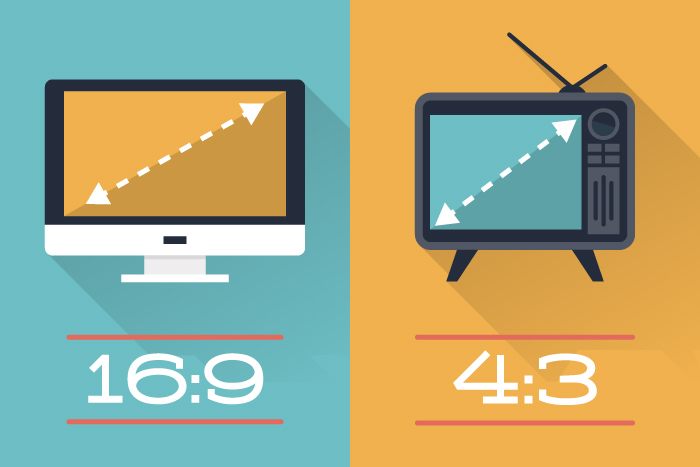
\includegraphics[width=0.7\textwidth]{img1/tvs}
\end{minipage}

 
	\exer  Si en una classe el 77,777{\dots} \% dels alumnes aproven i hi ha més de 30 alumnes però menys de 40, quants alumnes són i quants aproven? \textit{Ajuda: Passa $77,\hat{7}$ a fracció.}
 
\answers{$77,7...= \dfrac{700}{9}$; Són 36 alumnes en total dels quals aproven 28}


\vspace{-0.75cm}
	\exer  
	\begin{minipage}[t]{0.8\textwidth}
	Després dels resultats de la jornada de futbol d'aquest cap de setmana, el Osasuna ha jugat 24 partits, dels quals ha guanyat 6 i ha empatat els 5/12. Quants partits ha perdut? Quin percentatge representen els 6 partits guanyats sobre el total de partits jugats?
	\end{minipage}
	\begin{minipage}{0.2\textwidth}
		\centering
		\vspace{0.5cm}
		
\includegraphics[width=1.5cm]{img1/balon}
	\end{minipage}
\answers{Perden 8 partits (10 empatats). $\dfrac{6}{24}=25$ \%}


	\exer  Una fundació té un dipòsit de diners per premiar joves artistes. D'aquests diners, la meitat seran per al primer premi, la tercera part per al segon premi, la dotzena part per al tercer premi i els 2.000 € que, d'aquesta manera, sobren es reservaran per a properes edicions. Quants diners rebrà cada premiat ?
\answers{Total 24000 \euro{}; 1r: 12000 \euro{}, 2n: 8000 \euro{}, 3r: 2000 \euro{} }




	\exer  En una escola hi ha 1800 alumnes, dels quals 860 són noies. Els 3/4 de les noies i els 2/5 dels nois practiquen natació. Quants alumnes en total practiquen natació?

\answers{645 nines + 376 nins = 1021 alumnes practiquen natació.}



	\exer  Una empresa disposa de 7.200 € de pressupost mensual, del qual tres cinquenes parts es dediquen a pagar els sous dels treballadors, una quarta part a cobrir despeses comunes, i amb la resta es fa un fons d'estalvi per possibles imprevistos.


a ) Quina fracció del pressupost es destina a aquest fons d'estalvi? Quin percentatge del sou mensual representa?

b ) Quants diners s'han estalviat a l'acabar l'any ?

\answers{[$\dfrac{3}{20}=15$ \%, $12960$ \euro{}]}


	\exer  Una mare divideix el contingut d'una caixa de llepolies entre els seus tres fills; al primer li dóna la meitat del total, al segon, dues cinquenes parts del total, i al tercer, les 6 que queden. 


a) Quantes llepolies conté la caixa? 

b ) Quantes llepolies toquen a cada un dels fills?
\vspace{0.5cm}

\answers{La caixa conté 60 llepolies. Primer fill 30, segon fill 24 llepolies.}

\end{mylist}

\begin{example}[*]
	Entre els dos primers fills tindran $\frac{1}{2} + \frac{2}{5}= \frac{9}{10}$.
	%%
	Per tant, el tercer fill tindrà $1-\frac{9}{10}= \frac{1}{10}$.
	
	Sabem que aquesta fracció del total $x$ correspon a 6 llepolies.
	$\frac{1}{10} \text{ de } x = 6$ \quad $\rightarrow$ \quad $x=60$.
	
	Ara ja sabem que la caixa conté 60 llepolies. Sabries calcular quantes li toquen al primer i segon fill?
	
\end{example}

\pagebreak


\begin{mylist}
	
	\exer  Marta té 1.500 € al seu compte corrent. Gasta 1/3 en una cadena musical i 2/5 en una reparació del cotxe. Quants diners li queden?
\answers{100 \euro{}}




	\exer  A la selecció per a un concurs televisiu, passen la primera prova 5/12 dels aspirants i en la segona prova passen 4/13 dels que quedaven.


a ) Expressa en forma de fracció els aspirants que han estat seleccionats pel concurs.

b) Si 130 aspirants van passar la primera prova, quants aspirants es van presentar inicialment?
\answers{[7/39, Es van presentar 312 aspirants]}



	\exer   Per a la construcció d'un poliesportiu, l'Ajuntament aporta 1/10 del cost, la Unió Europea, 1/6 parts, el Govern, 4/15 parts, i la resta s'aconsegueix amb un préstec.


a ) Calcula la fracció del cost que representa el préstec.

b ) Si el Govern aporta 416.000 euros, calcula el cost total d'aquesta obra.

\answers{[7/15, 1.560.000 \euro{}]}


	\exer  Un alumne ha de llegir una novel·la en quatre setmanes. La primera setmana llegeix 5/12 de la novel·la, la segona setmana llegeix 5/24 i la tercera setmana llegeix 2/8 de la novel·la.


a ) Quina fracció de la novel·la ha de llegir la quarta setmana ?

b ) Si la novel·la té 216 pàgines, quantes ha llegit cada setmana ?
\answers{[1/8, 90; 45; 54; 27 cada setmana]}


	\exer  
	\begin{minipage}[t]{0.7\textwidth}	
	  Quantes botelles de 3/4 de litre necessit per tenir la mateixa quantitat que en 60 botelles de 3/5 de litre?
\end{minipage}
\begin{minipage}[t]{0.3\textwidth}
	\centering
	\vspace{-1.75cm}
	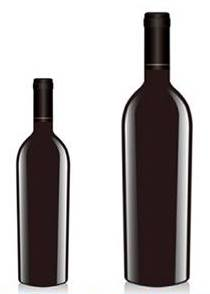
\includegraphics[width=0.4\textwidth,valign=t]{img1/botellas}
\end{minipage}
\answers{48 botelles}


	\exer  Troba un nombre enter de tal forma que: la seva meitat, la seva tercera part, la seva quarta part, la seva cinquena part, la seva sisena part i la seva setena part siguin nombres enters.
\answers{$2\times 3\times 4\times 5\times 6\times 7=5040$ o també 420.}






	\exer  A la unitat li llevo les seves dues cinquenes parts. Per quina fracció cal multiplicar el resultat per arribar una altra vegada a la unitat?
\answers{Cal multiplicar per la fracció $\dfrac{5}{3}$}




	\exer  Troba la fracció resultant:


a) Llevo 1 terç del que tinc i després afegeixo 1 terç del que queda.

b) Afegeixo 1 terç del que tinc i després llevo 1 terç del resultat.

\answers{[$\dfrac{8}{9}$, $\dfrac{8}{9}$]}




	\exer  Estàs avorrit i decideixes jugar al següent: Avances un metre en línia recta, retrocedeixes la meitat, avances la meitat del que has retrocedit en l'últim pas, retrocedeixes la meitat del que has avançat en l'últim pas, {\dots}


Si ho fas moltes, però que moltes vegades, quant avances en total?
\[1-\frac{1}{2} +\frac{1}{4} -\frac{1}{8} +\frac{1}{16} -\frac{1}{32} +...=\] 
\answers{2/3 de metre.}



\begin{comment}
	\exer  \includegraphics*[bb=0 0 1.24in 1.25in, width=1.24in, height=1.25in, keepaspectratio=false]{img1/image8.png} La figura del costat és un ``Tangram''.


a) Troba la fracció que es correspon amb cadascuna de les 7 peces.

b) Si el costat del quadrat és de 20 cm, troba l'àrea de cada peça.
\end{comment}

\end{mylist}


\pagebreak

\section{Aproximacions i errors}
 
\begin{theorybox}
Si d'una quantitat sabem el valor exacte i el valor aproximat, definim

L'error absolut és E${}_{A}$ = {\textbar}Valor exacte -- Valor aproximat{\textbar}

L'error relatiu és E${}_{R}$ = E${}_{A}$ / Valor exacte

Per exemple, si aproximem el número $\pi$ per 3,14 els errors comesos són:

E${}_{A}$ = {\textbar}$\pi$ -- 3,14{\textbar} =0,0016

E${}_{R}$ = 0,0016 / $\pi$ = 0,0005    =    0,05 \%

\end{theorybox}

\begin{mylist}
	\exer  \spen  Copia aquesta taula en el teu quadern i arrodoneix amb el nombre de xifres indicat


\begin{tabular}{|p{0.15\textwidth}|p{0.15\textwidth}|p{0.15\textwidth}|p{0.15\textwidth}|p{0.15\textwidth}|} \hline 
	\rowcolor{lightgray} \textbf{} & \multicolumn{4}{|p{2.5in}|}{\textbf{Xifres significatives}} \\ \hline 
	\textbf{Nombre} & 1 & 2 & 3 & 4 \\ \hline 
	\textbf{$\sqrt{10} $} &  &  &  &  \\ \hline 
	\textbf{1/7} &  &  &  &  \\ \hline 
	\textbf{95549} & 100000 &  &  &  \\ \hline 
	\textbf{30000} & 3·10${}^{4}$ &  &  &  \\ \hline 
	\textbf{1,9995} &  &  &  & 2,000 \\ \hline 
\end{tabular}
\answers{\begin{tabular}{|p{0.15\textwidth}|p{0.15\textwidth}|p{0.15\textwidth}|p{0.15\textwidth}|p{0.15\textwidth}|} \hline 
		\textbf{} & \multicolumn{4}{|p{0.6\textwidth}|}{Xifres significatives} \\ \hline 
		\textbf{Nombre} & 1 & 2 & 3 & 4 \\ \hline 
		\textbf{$\sqrt{10} $} & 3  & 3.2 & 3.16 & 3.162 \\ \hline 
		\textbf{1/7} & 0.1 & 0.14 & 0.143  & 0.1429 \\ \hline 
		\textbf{95549} & 100000 & 96000 & 95500 &  95550\\ \hline 
		\textbf{30000} & 3·10${}^{4}$ & 30·10${}^{3}$ & 300·10${}^{2}$ & 3000·10${}^{1}$  \\ \hline 
		\textbf{1,9995} & 2 & 2,0 & 2,00 & 2,000 \\ \hline 
\end{tabular}}


	\exer  Prova que 123,45 amb $E_A = 0,005$ i 0,12345 amb $E_A = 0,000005$ tenen el mateix $E_R$.
	\answers{Els dos tenen com $E_R=4.05\cdot 10^{-3}$}
	
	\exer  Contesta Vertader o Fals i justifica la teva resposta:


a) Per a una mateixa màquina, l'error comès és menor com més petita sigui la mesura.

b) No es poden comparar errors relatius de diferents magnituds.

c) Posar preus com 1,99 €/Kg és un intent d'engany.

d) Comprar a 1,99 €/Kg enfront de 2 €/Kg suposa un estalvi.

e) Posar moltes xifres en un resultat significa que un és un gran matemàtic.

f) La precisió es mesura pel nombre de xifres decimals.

\answers[cols=2]{[Depèn si $E_R$ o $E_A$, F, V, F, F, V]}


	\exer  Aproxima els nombres 32567 i 1,395 amb 2 xifres significatives i digues en quin es comet menor error relatiu.
	\answers{$32567=33000$ amb $E_R=0.013$ i $1,395=1,400$ amb $E_R=0.0036$}
	
	\exer  $\pi$ no pot representar-se mitjançant una fracció d'enters però, pots trobar una fracció que ho aproximi amb 5 xifres significatives? 
	\answers{$3.1416 = \dfrac{31416}{10000}=\dfrac{3927}{1250}$}
	
	\exer  Aproximem $\pi$ per $3+\frac{1}{7+\frac{1}{16} } $:
	

a) Simplifica fins a una fracció impròpia irreductible.

b) Troba l'error absolut i l'error relatiu.

\answers{[$\dfrac{355}{113}$, $E_A=2.67\cdot 10^{-7}$, $E_R=8.5\cdot 10^{-6}$]}

\end{mylist}


\newpage
\begin{autoaval}{51}

\begin{mylist}
	\exer[2]  Resol pas a pas: $(-8 - 7 \cdot (-4 + 6) : (2 + (-3)) + 5 - 4 · 2^{2}) \cdot (-2)$
	\answers{10}


	\exer[2] Ordena de major a menor:
	$\frac{5}{6} \, ;\frac{7}{8} ;\, \frac{-7}{8} ;\frac{-5}{6} ;\, \frac{-5}{4}$
	\answers{$\frac{7}{8}>\frac{5}{6}>\frac{-5}{6}>\frac{-7}{8}>\frac{-5}{4}$}
	
	\exer Representa sobre la recta numèrica:
	$\frac{3}{4} ;\, \frac{17}{6} ;\, \frac{-11}{7} ;\, -0,125$
	
	\exer[2]  Resol pas a pas i simplifica:
	$\frac{\frac{2}{3} -\frac{5}{6} :\left(2-\frac{11}{3} \right)}{\frac{2}{6} } $
	\answers{$\frac{7}{2}$}
	
	\exer[2]  
a) Troba les quatre cinquenes parts dels cinc vuitens de 360.

b) Una ampolla té plenes les seves set vuitenes parts, si conté 840 cm${}^{3}$, quant li cap plena?
	\answers{[180, 960 cm${}^3$]}

	\exer[2]  Aproxima els nombres 9859 i 9,945 amb 2 xifres significatives i calcula els errors relatius comesos (en \%), quin és menor?
	\answers[cols=1]{[9900,$E_A$=41,$E_R$=0.42\%, 9.9,$E_A$=0.045,$E_R$=0,45\% ]}
	
	\exer[2]

a) Digues quins de les següents fraccions tenen expressió decimal exacta i quins periòdica:  $\frac{6}{120} ;\, \frac{5}{180} ;\, \frac{42}{210} $

b) Quants decimals té $\frac{1}{2^{10} \cdot 5^{6} } $ ?

c) Quantes xifres com a màxim pot tenir el període d'1/97?
\answers{[Són exactes $\dfrac{6}{120}$ i $\dfrac{42}{150}$. $\dfrac{5}{180}$ és decimal periòdic, 10 xifres, 96 xifres]}

	\exer[2]  Passa a fracció i simplifica:

a) 2,225 \quad\quad\quad b) 2,2252525... \quad\quad\quad c) $\frac{0,125}{0,125125125...} $ 
\answers{$\frac{89}{40}$, $\frac{2203}{990}$, $\frac{999}{1000}=0,999$}

	\exer[2]

Una medusa creix cada setmana un terç del seu volum.

a) Quantes setmanes han de passar perquè el seu volum es multipliqui per més de 3?

b) Si el seu volum actual és de 1200 cm${}^{3}$, quin era el seu volum fa 3 setmanes?
\answers[cols=2]{[4 setmanes, 506.25 cm${}^{3}$]}

	\exer[2]  A un treballador li baixen el sou la sisena part, del que li queda el 25 \% es va destinat a imposts i finalment de la resta que \textbf{li queda} les dues cinquenes parts les hi gasta a pagar la hipoteca del pis. Si encara té disponibles 450 \euro{}, quant cobrava abans de la baixada de sou?, quant paga d'impostos i d'hipoteca?
	
	\answers{Cobrava 1200 \euro{}. Ara cobra 1000 \euro{}, paga 250 \euro{} d'impostos i 300 \euro{} d'hipoteca. }
\end{mylist}


\end{autoaval}












\newpage

\resum
 \begin{center}
 	\renewcommand{\arraystretch}{1.3}
\begin{longtable}{|p{0.54\textwidth}|p{0.39\textwidth}|} \hline 
	
	\rowcolor{lightgray}\multicolumn{2}{|p{\textwidth}|}{\bf Prioritat de les operacions} \\ \hline
	
	  1r  Parèntesis interiors                            
	  
	  2n Potències i arrels
	  
	  3r Productes i divisions                           
	  
	  4t Sumes i restes. & \[10 - 5 \cdot (4 - 3 \cdot 2^{2}) = 50 \] \\ \hline 
	  
	 	\rowcolor{lightgray}\multicolumn{2}{|p{\textwidth}|}{\bf Signe de la suma} \\ \hline 
	 (+) + (+) = (+) se sumen, 
	 
	 (--) + (--) = (--) se sumen.
	 
	  (+) + (--) = ? se resten i té el signe del més gran. & \[-\frac{7}{3} - \frac{8}{3} = -\frac{15}{3} = -5\] 
	  \[ -\frac{12}{5} + \frac{8}{5} = -\frac{4}{5}\] \\ \hline 
	
		\rowcolor{lightgray}\multicolumn{2}{|p{\textwidth}|}{\bf Signe del producte i la divisió} \\ \hline
 Si tenen igual signe dóna positiu.
 
  \quad (+)·(+) = (--)·(--) = (+)\newline Si tenen signe contrari dóna negatiu. 
 
 \quad (+)·(--) = (--)·(+) = (--) & --4 · (--10) = +40\newline
  +2 · (--15) = --30 \\ \hline 
	
		\rowcolor{lightgray}\multicolumn{2}{|p{\textwidth}|}{\bf Nombre racional} \\ \hline
	Un nombre  $r$ és racional si pot escriure's com a \linebreak \textit{r =$\frac{a}{b}$} amb \textit{a, b} enters i \textit{b}$\ne $ 0.\newline  & 2; \, --7/2 són racionals. També 2,6777... $\sqrt{2} \, i\, \, \pi $ no ho són. \\ \hline 
	
	
		\rowcolor{lightgray}\multicolumn{2}{|p{\textwidth}|}{\bf Fracció irreductible} \\ \hline
	S'obté dividint el numerador i el denominador pel mateix nombre. Numerador i denominador són primers entre si. & \[ \frac{360}{840} = \frac{3}{7} \]  l'última és irreductible. \\ \hline 
	
		\rowcolor{lightgray}\multicolumn{2}{|p{\textwidth}|}{\bf Fraccions equivalents} \\ \hline
  Són equivalents les fraccions que tenen igual expressió decimal. Dues fraccions equivalents representen al mateix nombre racional. Els seus productes creuats valen el mateix. & \[\frac{{\rm 3}}{{\rm 4}} {\rm =}\frac{{\rm 6}}{{\rm 8}} {\rm =}\frac{{\rm 15}}{{\rm 20}} = 0,75\] són equivalents: $3 \cdot 8 = 4 \cdot 6$ \\ \hline 
	
		\rowcolor{lightgray}\multicolumn{2}{|p{\textwidth}|}{\bf Ordenar fraccions} \\ \hline
 Es passen a comú denominador o es troba el seu valor decimal o s'usa la lògica i el truc $\frac{a}{b}<\frac{c}{d}$ si $a\cdot d < b\cdot c$ per a nombres positius. & \[\frac{3}{4} <\frac{4}{5} <\frac{9}{10} \, \text{ ja que } \, \frac{15}{20} <\frac{16}{20} <\frac{18}{20} \] \\ \hline 
	  \newpage
		\rowcolor{lightgray}\multicolumn{2}{|p{\textwidth}|}{\bf Representació sobre la recta numèrica} \\ \hline
  Si és necessari es passen a forma mixta. Per a  \linebreak $n + {a/b}$ dividim la unitat que va de $n$ a   $n + 1$ en  $b$ parts iguals i prenem $a$ trossos.  Per a $-\textit{n} - \textit{a/b}$ dividim la unitat que va de $-\textit{n}$ a $-\textit{n} - 1$ en  $b$ parts iguals i comptem $a$ començant en $-\textit{n}$. & \begin{center}\includegraphics*[bb=0 0 2.00in 0.67in, width=2.00in, height=0.67in, keepaspectratio=false]{img1/image9.png}\end{center} \\ \hline 
	
		\rowcolor{lightgray}\multicolumn{2}{|p{\textwidth}|}{\bf Suma i resta de fraccions} \\ \hline
	  Es passen a comú denominador i se sumen (resten) els numeradors. & \[\frac{5}{6} -\frac{7}{8} =\frac{20}{24} -\frac{21}{24} =\frac{-1}{24} \] \\ \hline 
	
	
		\rowcolor{lightgray}\multicolumn{2}{|p{\textwidth}|}{\bf Producte i divisió de fraccions} \\ \hline
	  
	  \[ \frac{a}{b} \cdot \frac{c}{d} = \frac{a\cdot c}{ b\cdot d} \]
	    \[ \frac{a}{b} : \frac{c}{d} = \frac{a\cdot d}{ b\cdot c} \]
	  
	    & \[ \frac{2}{7} \cdot \frac{14}{6} =\frac{2\cdot 2\cdot 7}{7\cdot 2\cdot 3} =\frac{2}{3} \] \[ \frac{6}{5} :\frac{14}{10} =\frac{6}{5} \cdot \frac{10}{14} =\frac{6}{7} \]   \\ \hline 
	
		\rowcolor{lightgray}\multicolumn{2}{|p{\textwidth}|}{\bf Fracció d'una quantitat} \\ \hline
	 \[ \frac{a}{b} \text{ de } x = \frac{a}{b} \cdot x = \frac{a\cdot x}{b} \] & \[ \frac{3}{4} \text{ de } 60 = \frac{3}{4} \cdot 60 = 45 \] \[ \frac{3}{4} \text{ de } \frac{4}{5} =  \frac{3}{4}\cdot  \frac{4}{5} =  \frac{3}{5} \]  \\ \hline 
	
	
		\rowcolor{lightgray}\multicolumn{2}{|p{\textwidth}|}{\bf Errors} \\ \hline
	 Error absolut:\newline \quad $E_A = \left|valor\, real\, -\, valor\, aproximat\right|$\newline Error relatiu: $E_R = \frac{E_A}{\left|Valor\, real\right|} $ es multiplica per 100 per obtenir-ho en \%. & $\begin{array}{l} {\frac{2}{3} \approx 0,7\Rightarrow E_A\approx 0,033} \\ {\Rightarrow E_R\approx \frac{0,033}{2/3} \approx 0,050\Rightarrow 5\% } \end{array}$ \\ \hline 
	
		\rowcolor{lightgray}\multicolumn{2}{|p{\textwidth}|}{\bf Fraccions i decimals} \\ \hline
	 L'expressió decimal d'una fracció sempre és exacta o periòdica. Exacta si el denominador només té com a factors primers el 2 o el 5. Periòdica en cas contrari. & 3/40 = 0,075 exacte \newline 1/3=0,3333... periòdic pur \newline 5/12 = 0,41666... periòdic mixt \\ \hline 
	
		\rowcolor{lightgray}\multicolumn{2}{|p{\textwidth}|}{\bf Pas de decimal a fracció} \\ \hline
  Expressió decimal exacta: es divideix el nombre sense la coma entre la unitat seguida de punts zeros com a xifres decimals. \newline Expressió decimal periòdica: Es multiplica \textit{N} per potències de \textit{10} fins aconseguir 2 nombres amb la mateixa part decimal, es resten i s'aïlla \textit{N.} & $3,175 = \frac{3175}{1000} = \frac{127}{40}$\newline\newline \textit{N }= 2,033...  100\textit{N} - 10\textit{N} = 183\newline 90\textit{N }= 183  $\textit{N} = \frac{183}{90}=\frac{61}{30}$. \\ \hline 
\end{longtable}
 
\end{center}

 